\documentclass[french,11pt,twoside]{VcCours}

%cSpell:ignore SGBD BDDR Ellison Comyn Wattiau Akoka Balabonski Roadtrip Beautiful Journey Viva Playa Codd
\begin{document}

\Titre{PSI}{Promotion 2021--2022}{Informatique}{TP d'info n°8 -- Bases de données.}

\tableofcontents
\separationTitre

% Le stockage, l'organisation et l'utilisation de données (de nature aussi variée 
% que des textes, des valeurs numériques, des images, des vidéos, ...) constituent 
% l'un des piliers de l'informatique, en tant que science du traitement de 
% l'information. Des ensembles cohérents et structurés de données stockées sur un 
% support persistant sont appelés \emph{bases de données}. Elles jouent un rôle 
% fondamental dans la majorité des organisations économiques, scientifiques, 
% culturelles et institutionnelles. Par exemple, toute entreprise dispose d'une 
% base de données, ne serait-ce que pour gérer ses stocks de marchandises et ses 
% clients avec leur commandes. A l'heure actuelle, on estime le marché annuel 
% pour les systèmes de gestion des bases de données (SGBD) à plusieurs dizaines 
% de milliards d'euros. Autre chiffre impressionnant : Larry Ellison, le 
% cofondateur d'Oracle, spécialisé dans les SGBD, est, en septembre 2020, 
% le 8eme homme le plus riche du monde avec 80 milliards de dollars ! Dans le 
% cadre du programme de NSI Terminale, le présent document a pour but de justifier 
% de l'intérêt informatique et pratique d'utiliser des bases de données (BDD), 
% de présenter le modèle le plus courant de BDD (modèle dit relationnel) et les 
% SGBD associés et de comprendre comment manipuler, interroger et mettre à jour 
% une BDD au moyen du langage SQL.

% Quelques références bibliographiques :
% \begin{itemize}
%  \item \emph{Les bases de données}, I. Comyn-Wattiau et J. Akoka, P.U.F, collection Que sais-je ?, 2003
%  \item Le Portail Wikipédia \emph{Bases de données}, \url{https://fr.wikipedia.org/wiki/Portail:Bases_de_donnees}
%  \item MOOC (archivé) \emph{Bases de données relationnelles : apprendre pour utiliser}, plateforme FUN Mooc, \url{https://www.fun-mooc.fr}
%  \item \emph{Numérique et sciences informatiques, Terminale}, T. Balabonski et al., éditions Ellipses, 2020
%  \item SQL.sh (cours et tutoriels sur le langage SQL), \url{https://sql.sh/}
% \end{itemize}


% %%%%%%%%%%%%%%%%%%%%%%%%%%%%%%%%%%%%%%%%%%%%%%%%%%%%%%%%%%%%%%%%%%%%%%%%%%
% \section{Limitations des tableaux}
% %%%%%%%%%%%%%%%%%%%%%%%%%%%%%%%%%%%%%%%%%%%%%%%%%%%%%%%%%%%%%%%%%%%%%%%%%%

% Lorsqu'on veut stocker des données simples (textes, valeurs numériques, booléens, ...), la première structure qu'on envisage est en général un tableau. Un tel tableau possède plusieurs colonnes, chaque colonne ayant un titre, et plusieurs lignes, chaque ligne faisant référence à une entité ayant les caractéristiques définies par les colonnes. Par exemple, le tableau suivant représente des séjours de vacance proposés par un voyagiste.

% \begin{center}
% \begin{tabular}[c]{l|l|l|l|l|l|l}
% Dénomination & Pays & Type & Départ & Durée & Prix & Organisateur local \\ \hline
% Sur les routes d'Écosse & Écosse & Roadtrip & 03/04/2022 & 7 jours & 1000 & BeautifulJourney \\
% Sur les routes d'Espagne & Espagne & Roadtrip & 03/04/2022 & 8 jours & 850 & VivaLaPlaya \\
% L'île de Ré & France & Séjour & 30/05/2022 & 14 jours & 2300 & FranceVoyage \\
% Les vignobles bordelais & France & Circuit & 14 juin 2022 & 1 semaine & 1200 & FranceVoyage \\
% Sur les routes d'Écosse & Écosse & Roadtrip & 04/05/2022 & 7 minutes & 1150 & BeautifulJourney
% \end{tabular}
% \end{center}

% Des informations pertinentes y sont écrites. Cependant, plusieurs inconvénients et problèmes se posent : 
% \begin{itemize}
%  \item Une même dénomination peut désigner plusieurs voyages (par exemple à des dates différentes)
%  \item Des informations relatives à une même colonne peuvent être écrites de différentes façons, parfois de manière erronée (ex : "7 minutes" pour la durée du dernier voyage)
% \end{itemize}
% Bref des risques d'anomalie et d'incohérence sont possibles en insertion, modification et suppression de données. D'autre part, il n'est pas possible de faire des recoupements intéressants avec d'autres tableaux éventuels. Par exemple, avec un tableau de données météorologiques qui donnerait les températures moyennes et les précipitations attendues dans tel pays à tel date ; c'est pourtant une question fréquente pour un touriste en vue de choisir un voyage agréable. Enfin, d'autres problèmes peuvent se poser : 
% \begin{itemize}
%  \item Les données peuvent être présentes sur différents ordinateurs, localisés dans différentes villes où sont situées les agences du voyagiste.  Que se passe-t-il si un agent modifie  ou ajoute un nouveau voyage avec son ordinateur ? Cela devrait être répercuté sur les autres jeux de données des autres agences.
%  \item Si deux agents modifient en même temps un voyage, qui a la priorité de la mise à jour ?
%  \item Comment éliminer tous les voyages proposés par un organisateur local qui a fait faillite ?
%  \item Comment gérer des tableaux à plusieurs millions de lignes, rapidement et avec une occupation mémoire raisonnable ?
% \end{itemize}

% Des structures de données plus ingénieuses, associées à des logiciels spécifiques, ont donc été conçues pour résoudre tout ou partie de ces problèmes. Ce sont les bases de données (BDD). Parmi elles, les bases de données dites relationnelles sont les plus courantes et constitueront le cœur de ce cours. Le modèle relationnel a été proposé par l'américain Edgar Codd en 1970, mais il reste à l'heure actuel le modèle le plus utilisé.


% \subsubsection*{Activité 1}

% Citer des systèmes, des services, des organisations, des sites Internet qui utilisent des bases de données.

% % Amazon, data.gouv.fr, INSEE, un GPS, un carnet d'adresses d'un smartphone (et nbreux autres ex avec les smartphones !!) ...


%%%%%%%%%%%%%%%%%%%%%%%%%%%%%%%%%%%%%%%%%%%%%%%%%%%%%%%%%%%%%%%%%%%%%%%%%%
\section{Bases de données relationnelles}
%%%%%%%%%%%%%%%%%%%%%%%%%%%%%%%%%%%%%%%%%%%%%%%%%%%%%%%%%%%%%%%%%%%%%%%%%%

\subsection{Modèle et vocabulaire}

\begin{Definition}{}
Une base de données relationnelle (BDDR) est un ensemble fini de tableaux à deux dimensions, appelés \emph{relations} (ou parfois \emph{tables}). Chaque relation porte un \emph{nom}. Chaque relation admet un ensemble fini de colonnes, appelées \emph{attributs} (ou parfois \emph{champs}). Chaque attribut admet un type (chaîne de caractères, entier, booléen, ...) appelé \emph{domaine}. D'autre part, une relation admet un nombre fini de lignes : chaque ligne d'une relation définit une entité\footnote{qui peut représenter concrètement un objet physique, une personne, une action, une entreprise, un lieu, une organisation, ...} appelée \emph{n-uplet} (en anglais \emph{tuple}) ; on parle aussi d'\emph{enregistrement} (en anglais \emph{record}). Un n-uplet est identifié de manière unique dans une relation grâce à un attribut (ou un ensemble d'attributs) appelé \emph{clé primaire}\footnote{Une clé primaire d'une table, utilisée par une autre table, est appelée \emph{clé étrangère} dans cette deuxième table ; elle permet d'établir ainsi une connexion entre deux tables. C'est un atout fondamental des BDD par rapport à de simples tableaux déconnectés.}.
\end{Definition}



\begin{figure}[ht]
\centering
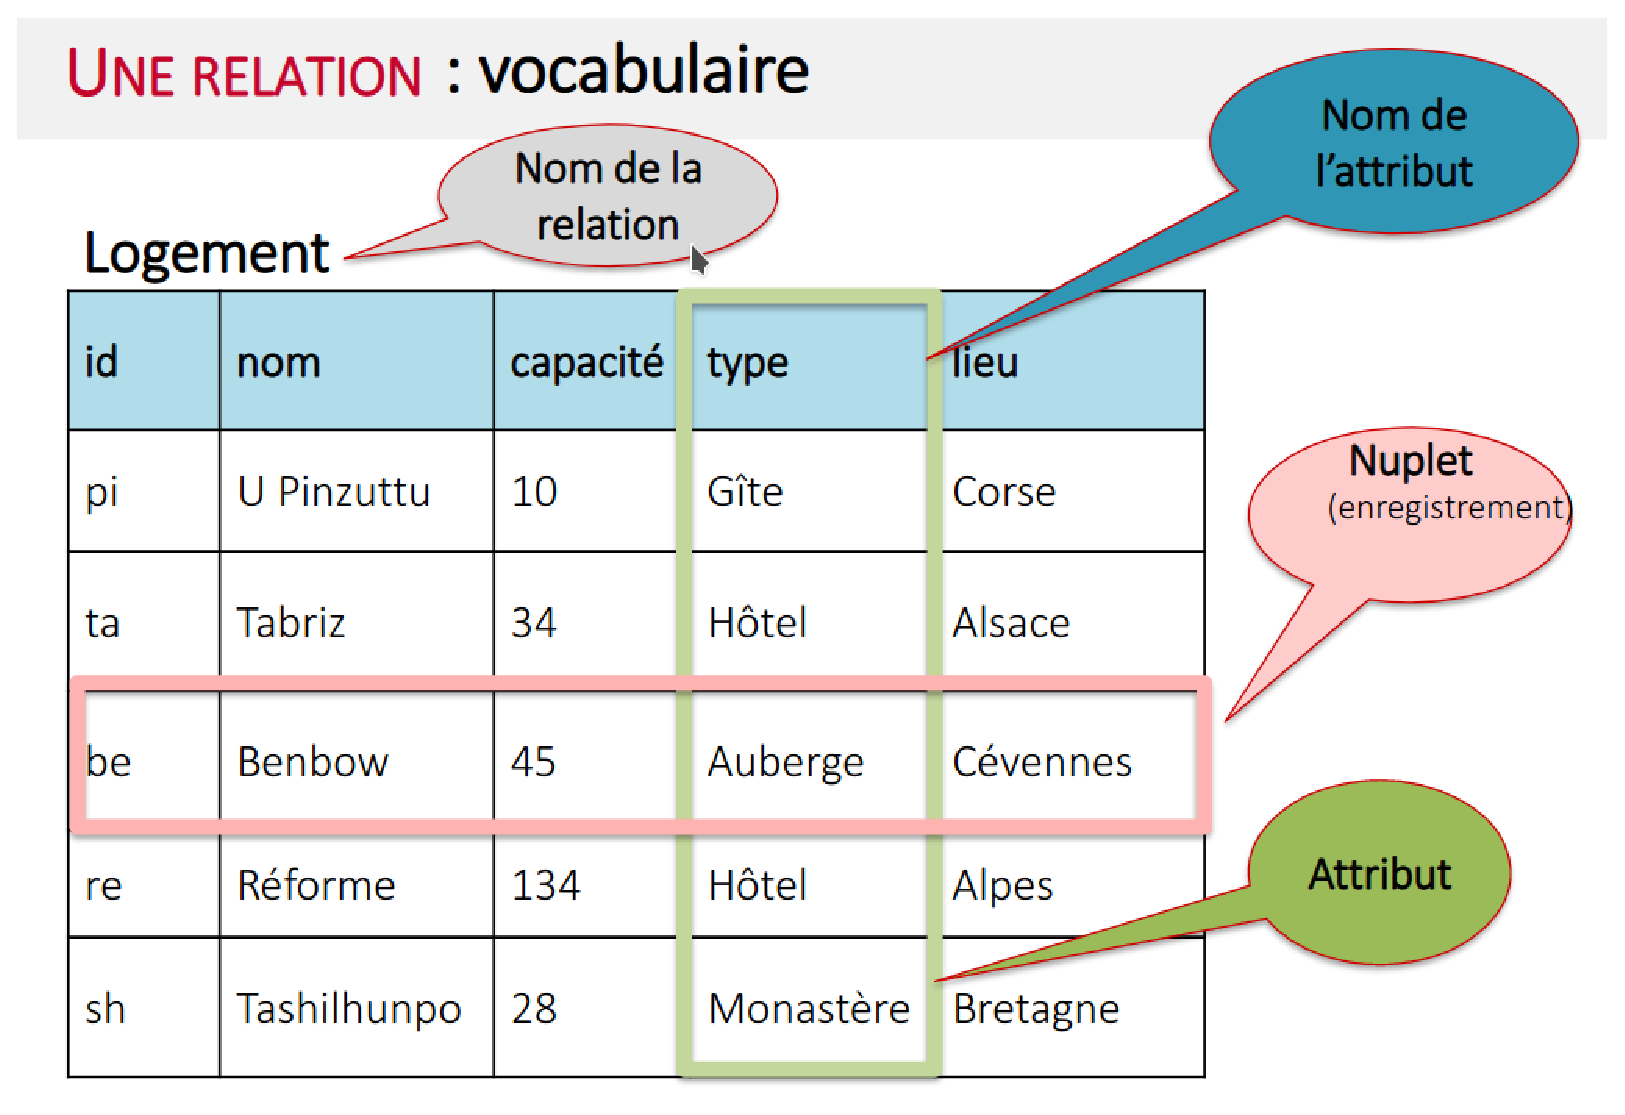
\includegraphics[width=12cm]{voca_graphique.eps}
\end{figure}


% 
% {%
% \newcommand{\mc}[3]{\multicolumn{#1}{#2}{#3}}
% \begin{center}
% \begin{tabular}{|l|l|l|} \hline
% \mc{3}{|c|}{Etudiants}\\ \hline
% \textbf{Id} & Nom & Prénom\\ \hline
% Int & String & String\\ \hline
% \end{tabular}
% \end{center}
% }%
% 
% {%
% \newcommand{\mc}[3]{\multicolumn{#1}{#2}{#3}}
% \begin{center}
% \begin{tabular}{|l|l|l|l|} \hline
% \mc{4}{|c|}{Groupes\_de\_colle}\\ \hline
% \textbf{Id} & Etudiant1 & Etudiant2 & Etudiant3\\ \hline
% Int & Int & Int & Int\\ \hline
% \end{tabular}
% \end{center}
% }%
% 

Finalement, une BDDR se définit par un \emph{schéma relationnel}, c'est-à-dire la structure générale de cette BDD : c'est un modèle, une représentation simple et synthétique, définissant une base de données par un ensemble de relations, où chaque relation est caractérisée par un ensemble d'attributs, avec un domaine précisé pour chacun. 

Par exemple, on peut définir une BDDR relative à la gestion d'une classe de CPGE (où se déroulent des oraux appelés "colles") avec deux relations :
\begin{itemize}
 \item Etudiants(\textbf{Id} Int, Nom String, Prenom String)
 \item Groupes\_de\_colle(\textbf{Id} Int, IdEtudiant1 Int, IdEtudiant2 Int, IdEtudiant3 Int)
\end{itemize}

L'attribut en gras représente la clé primaire de la relation. A noter que IdEtudiant1, IdEtudiant2, IdEtudiant3 seront des clés étrangères (pas de symbole particulier) dans la mesure où ces valeurs correspondront à des Id de la base Etudiants, où cet attribut est une clé primaire.

Le schéma relationnel d'une BDD ne doit pas être confondu avec l'\emph{instance} de cette base de données, qui est l'ensemble des n-uplets (ayant une même structure), autrement dit qui indique le jeu de valeurs contenues dans la BDD. Ex :

\begin{multicols}{2}
{%
\newcommand{\mc}[3]{\multicolumn{#1}{#2}{#3}}
\begin{center}
\begin{tabular}{|l|l|l|} \hline
\mc{3}{|c|}{\textsc{Etudiants}}\\ \hline
\textbf{Id} & Nom & Prenom\\ \hline
0 & ' ' & ' ' \\ \hline
1 & 'DeLaRue' & 'Toto' \\ \hline
2 & 'Chouette' & 'Léa' \\ \hline
3 & 'Tudors' & 'Zoé' \\ \hline
\end{tabular}
\end{center}
}%

{%
\newcommand{\mc}[3]{\multicolumn{#1}{#2}{#3}}
\begin{center}
\begin{tabular}{|l|l|l|l|} \hline
\mc{4}{|c|}{\textsc{Groupes\_de\_colle}}\\ \hline
\textbf{Id} & IdEtudiant1 & IdEtudiant2 & IdEtudiant3\\ \hline
1 & 3 & 1 & 2\\ \hline
\end{tabular}
\end{center}
}%
\end{multicols}

Concevoir une base de données est un travail en général complexe. Il existe des méthodes rigoureuses et des outils pour proposer des modèles respectant un cahier des charges imposé, afin de choisir au mieux l'organisation des données sous forme de relations judicieuses, en vue de leur utilisation, de leur stockage, ... Mais cela dépasse le cadre de ce cours.



\subsection{Grands principes des BDDR}

Les BDDR vérifient trois grands principes, qui justifient leur efficacité et leur succès.

\subsubsection{Universalité}

Les BDDR sont conçues pour gérer toutes les données possibles d'une entreprise ou d'un organisme, tous les utilisateurs possibles, toutes les applications possibles. Elle permettent de trouver et d'ajouter des informations pertinentes, de gérer des transactions simples ou complexes, dans des volumes importants, et d'analyser des données.

\subsubsection{Abstraction}

Ce concept comprend deux aspects :
\begin{itemize}
 \item L'utilisateur voit les données comme des tableaux à 2 dimensions, en ignorant les détails de leur organisation réelle sur disque (ou tout autre stockage mémoire).
 \item Les données sont manipulées avec des langages de haut niveau (tels que le langage SQL, mais aussi l'algèbre relationnelle, le calcul relationnel, des langages graphiques, ...)
\end{itemize}


\subsubsection{Indépendance}

Cela concerne les trois niveaux qu'implique une BDD : 
\begin{itemize}
 \item le niveau physique : la façon dont les données sont organisées au niveau des disques mémoire
 \item le niveau logique, avec les tableaux à deux dimensions et leurs connectivités
 \item le niveau externe, avec des \emph{vues} adaptées à chaque utilisateur (interface graphique, débugueur, ...)
\end{itemize}
Le fait qu'il y ait indépendance entre ces trois niveaux permet une très grande souplesse pour modifier, améliorer, optimiser une base de données en fonction d'un cahier des charges et de contraintes particulières.

\subsection{Contraintes vérifiées par les BDDR}

Il est fondamental qu'une BDDR respecte certaines contraintes dites d'intégrité, pour que la base de donnée fonctionne correctement et soit en accord avec les grands principes. Ces contraintes sont des propriétés logiques invariantes que les données doivent vérifier à tout instant. On cite essentiellement quatre types de contraintes :
\begin{itemize}
 \item Les contraintes d'entité : chaque entité d'une relation doit être unique. C'est le rôle joué par les clés primaires.
 \item Les contraintes de référence : cela concerne les données partagées entre deux (ou plus) relations. Une table qui fait référence à une entité d'une autre table doit s'assurer que cette entité existe bien et qu'elle est unique. C'est le rôle joué par les clés étrangères.
 \item Les contraintes de domaine : elles restreignent les valeurs d'un attribut à celles du domaine spécifié. Elles évitent d'ajouter (ou de modifier) un n-uplet dont une valeur n'est pas en accord avec le domaine d'un attribut. Dans la suite du cours, sauf contre-indication, on se restreindra aux 6 domaines suivants : String, Int, Boolean, Float, Date, Time.
 \item Les contraintes utilisateurs : ce sont des contraintes supplémentaires personnalisées, portant sur les valeurs des attributs (par ex, restreindre l'âge d'une personne à une valeur comprise entre 0 et 130, ou encore imposer d'avoir un symbole arobase dans une adresse mail).
\end{itemize}


\subsubsection*{Activité 1}

On considère la base de données d'un garagiste, avec une relation \emph{Voiture}, une relation \emph{Client} et une relation \emph{Possession} (dont la clé primaire est le couple (IdClient, IdVoiture)). Plusieurs anomalies ont été introduites à cause d'un bug logiciel du SGDB. Identifiez-les.

\begin{multicols}{3}

{%
\newcommand{\mc}[3]{\multicolumn{#1}{#2}{#3}}
\begin{center}
\begin{tabular}{|l|l|} \hline
\mc{2}{|c|}{\textsc{Voiture}}\\ \hline
\textbf{Id} (Int) & Modele (String)\\ \hline
1 & Renault Twingo\\ \hline
2 & Citroen C3\\ \hline
3 & Peugeot 2008\\ \hline
3 & Nissan Leaf\\ \hline
\end{tabular}
\end{center}
}%

{%
\newcommand{\mc}[3]{\multicolumn{#1}{#2}{#3}}
\begin{center}
\begin{tabular}{|l|l|} \hline
\mc{2}{|c|}{\textsc{Client}}\\ \hline
\textbf{Id (Int)} & Nom (String)\\ \hline
14 & Albert\\ \hline
2 & Freddy\\ \hline
client3 & Momo\\ \hline
\end{tabular}
\end{center}
}%

{%
\newcommand{\mc}[3]{\multicolumn{#1}{#2}{#3}}
\begin{center}
\begin{tabular}{|l|l|} \hline
\mc{2}{|c|}{\textsc{Possession}}\\ \hline
\textbf{IdClient} (Int) & \textbf{IdVoiture} (Int)\\ \hline
14 & 1\\ \hline
14 & 2\\ \hline
2 & 2\\ \hline
3 & 3\\ \hline
\end{tabular}
\end{center}
}%

\end{multicols}
% pour la table Voiture, 2 n-uplets ont la mm clé primaire
% pour la table Client, l'Id de Momo n'a pas le bon type
% pour la table Possession, l'IdClient 3 ne correspond à aucun Id de la table Client ; d'autre part, 2 clients possèdent la mm voiture d'Id 2 !

\subsubsection*{Activité 2} % d'ap exo 144 p 296 Ellipse NSI T

On veut concevoir une BDD portant sur les départements français. Elle doit stocker le nom, le code, le chef-lieu et la liste des départements voisins. Proposer un modèle relationnel. Attention le code d'un département peut s'écrire 07 (Ardèche), 2A (Corse du Sud) ou encore 971 (Guadeloupe). Attention, les listes ne font pas partie des domaines possibles pour les BDDR ! 

% réponse : avoir une relation "Département" (la clé primaire est le code du département) et une relation "Voisins", qui liste les couples de département limitrophes. Attention, il y aura forcément des doublons dans cette 2eme table. D'où l'idée d'imposer une contrainte utilisateur, par ex, en se limitant aux couples (code1, code2), avec code1 < code2 (ordre alphanumérique).


% \subsection{Systèmes de Gestion de Bases de Données (SGBD)}

% \begin{Definition}{}
% Un SGDB est un logiciel qui gère les données d'une base de données. 
% \end{Definition}

% C'est un logiciel complexe, avec souvent plusieurs centaines de milliers de lignes de code, installé sur un ou plusieurs ordinateurs, éventuellement distants géographiquement, qui gère des volumes de données très importants (plusieurs Go, voire To) et des partages multiples. 

% Un SGDB est basé sur une architecture client/serveur. Le SGDR reçoit des commandes de la part d'utilisateurs ou de systèmes informatiques, appelés \emph{clients}. Ces clients n'ont pas d'accès direct aux données de la base de données. C'est le SGDB qui va lire et interpréter la commande, exécuter cette commande en accédant à la BDD, et renvoyer le résultat au client (ou éventuellement un message d'erreur).

 

% \begin{figure}[ht]
% \centering
% \includegraphics[width=10cm]{clientserveur.eps}
% \end{figure}

% Un SGDB fournit des services aux clients, parmi lesquels on peut citer : 
% \begin{itemize}
%  \item la persistance des données : les données doivent être stockées sur des supports matériels, de manière pérenne, fiable. On doit pouvoir les récupérer en cas de défaillance matérielle ou logicielle.
%  \item la gestion des accès concurrents : il faut traiter et prioriser les accès simultanés de plusieurs clients, en gérant les éventuels conflits (un client peut vouloir accéder à une table alors qu'un autre est en train de l'effacer)
%  \item le traitement des requêtes : il faut interpréter la commande envoyée par un client. Cette commande est écrite dans un langage normalisé appelé SQL.
%  \item la sécurisation des accès : certaines données peuvent être sensibles (dossiers médicaux, secrets défense, secrets industriels ...). Il faut donc gérer des accès avec identifications et mots de passe et interdire toute autre intrusion susceptible de lire ou de corrompre les données.
% \end{itemize}
% On comprend bien que ces services sont intimement liés aux grands principes des SGBD et aux contraintes associées, afin d'assurer la cohérence des données.


% \subsubsection*{Activité 4}

% Rechercher sur Internet des noms de célèbres SGBD. Sont-ils libres ou propriétaires ? 

% MariaDB (libre), PostGreSQL (libre), Microsoft Access (proprio), ...
% liste exhaustive sur https://fr.wikipedia.org/wiki/Système_de_gestion_de_base_de_données

%%%%%%%%%%%%%%%%%%%%%%%%%%%%%%%%%%%%%%%%%%%%%%%%%%%%%%%%%%%%%%%%%%%%%%%%%%
\section{Langage SQL}
%%%%%%%%%%%%%%%%%%%%%%%%%%%%%%%%%%%%%%%%%%%%%%%%%%%%%%%%%%%%%%%%%%%%%%%%%%

Le langage SQL (sigle anglais pour Structured Query Language, c'est-à-dire langage de requête structuré) est un langage de haut niveau, jouant le rôle de médiateur entre les humains et les BDDR. Il est facilement compréhensible par les humains (du moins par les anglophones !), il est interprétable par un SGBDR, et il est même utilisé par les SGBDR pour communiquer entre eux ! Par convention, les mots-clé du langage SQL seront notés en majuscule (mais en fait l'interpréteur SQL ne tient pas compte de la casse, sauf pour les données des n-uplets). En revanche, il ne faut pas placer d'espaces pour les noms des tables et des attributs ; pour contourner cette contrainte, on utilise le caractère underscore ('\_'). De même, on évitera tout caractère accentué ou spécial (qui peut être mal géré par le SGBDR, s'il n'est pas paramétré avec un encodage adapté).

\subsection{Types de données en SQL}

SQL prend en charge de nombreux types de données,
%\footnote{Malheureusement, les différentes implémentations du langage SQL dans les SGBD ne respectent pas toujours parfaitement les normes, ce qui pose des problèmes de compatibilité et d'inter-opérabilité ...}
qui serviront de domaine aux attributs présents dans une table d'une BDD. On ne liste ci-après que les plus utiles.

\begin{center}
\begin{tabular}[c]{|l|r|} \hline
Type SQL & Description\\ \hline
INTEGER (ou INT) & Entier signé sur 32 bit\\ \hline
DECIMAL(t, f) & Nombre décimal avec t chiffres avant la virgule et f chiffres après\\ \hline
REAL & Flottant codé sur 32 bits\\ \hline
VARCHAR(n) & Chaîne de caractères avec au maximum n caractères\\ \hline
TEXT & Chaîne de caractères de taille quelconque\\ \hline
DATE & Date au format 'AAAA-MM-JJ'\\ \hline
TIME & Heure au format 'hh:mm:ss'\\  \hline
\end{tabular}
\end{center}


\subsection{Création d'une relation dans une base de données}

Cela est réalisé par la commande \verb'CREATE TABLE'. Par exemple, si le schéma relationnel s'écrit : 
Carnet(Prenom String, Nom String, Ville String, Naissance Date, Telephone String)
alors on écrira :
\begin{verbatim}
CREATE TABLE Carnet (Prenom VARCHAR(70), Nom VARCHAR(100), 
                     Ville VARCHAR(120), Naissance DATE,
                     Telephone String PRIMARY KEY);
\end{verbatim}
Plusieurs remarques : 
\begin{itemize}
 \item Le concepteur de BDD doit choisir les types SQL les plus adéquats par rapport aux domaines des attributs définis dans le schéma relationnel et anticiper la gamme de valeurs que prendront ces attributs dans les n-uplets.
 \item L'attribut Telephone n'a pas le type INT car les numéros de téléphone commencent en général par 0. Or un entier ne commence jamais pas un zéro (un message d'erreur serait retourné de toute façon). Seul un type chaîne de caractères peut convenir.
 \item Lors de la création de la table, il faut obligatoirement définir la clé primaire. On utilise la commande \verb'PRIMARY KEY' à la suite d'un attribut. Comme chaque personne a un numéro de téléphone qui lui est propre, cet attribut peut jouer parfaitement le rôle d'une clé primaire (alors que ce ne serait sans doute pas possible avec le nom de famille (qui est commun à tous les membres d'une même famille !). %Enfin, pour faire référence à une clé étrangère, il faudra utiliser la commande \verb'REFERENCES'.
 \item Lors de l'exécution d'une commande SQL, des vérifications sont automatiquement lancées par le SGBDR (par ex, la table Carnet ne doit pas exister, ou bien encore il faut avoir précisé une clé primaire).
\end{itemize}


\subsection{Modifications d'une base de données}

Pour supprimer une table d'une BDD, on utilise la commande \verb'DROP TABLE' ("drop" signifie lâcher, larguer en anglais). Par exemple : 
\begin{verbatim}
DROP TABLE Carnet;
\end{verbatim}
Toutes les données de la table Carnet seront également supprimées. Cependant, si un attribut de cette table sert de clé étrangère dans une autre table, cette opération de suppression sera interdite par le SGDBR. La conséquence est qu'il faut en général supprimer différentes tables dans un ordre bien précis, pour éviter une interdiction de suppression.

Pour inserer de nouvelles valeurs (sous forme de n-uplets), on utilise la commande \verb'INSERT INTO'. Par exemple :
\begin{verbatim}
INSERT INTO Carnet VALUES ('Toto', 'Atchoum', 'Paris', 2000-01-01, '0123456789'),
                          ('Zara', 'Youhou', 'Toulouse', 2000-02-02, '0122334455');
\end{verbatim}

Attention, des vérifications sont effectuées lors des opérations d'insertion, de sorte que les diverses contraintes (de domaine, d'utilisateur, ...) doivent être respectées, sous peine d'annulation de l'opération, avec génération d'un message d'erreur.


\subsection{Requêtes SQL d'interrogation et de mise à jour}


On considère une base de données d'une bibliothèque de ville. Elle possède plusieurs relations, selon le schéma relationnel :
\begin{itemize}
 \item Livre(Titre String, Editeur String, Annee Int, \textbf{CodeISBN} String) 
 \item Abonne(prenom String, ville String, email String, \textbf{NumAbonne} String)
 \item Emprunt(\textbf{CodeISBN} String, \textbf{NumAbonne} String, DateRetour Date)
\end{itemize}
Elle va servir de support pour les exemples de requêtes SQL. On liste ci-après les principales commandes et mots-clés SQL.


\subsubsection*{SELECT ... FROM ...}

C'est la commande primordiale pour sélectionner des données dans une BDDR. Sa syntaxe est :
\begin{verbatim}
SELECT nom_des_attributs FROM nom_de_la_table
\end{verbatim}
Par exemple,
\begin{verbatim}
SELECT Titre FROM Livre
\end{verbatim}
sélectionne (et affiche sur console SQL du SGDBR) tous les titres de tous les livres de la bibliothèque (il peut y avoir des doublons, s'il y a plusieurs exemplaires d'un livre). A priori, l'affichage n'est pas ordonné.
\begin{verbatim}
SELECT CodeISBN, Editeur FROM Livre
\end{verbatim}
sélectionne le code ISBN et l'éditeur de chaque livre.
\begin{verbatim}
SELECT * FROM Livre
\end{verbatim}
sélectionne la totalité de la table Livre, ce qui permet de "voir" facilement ce qu'elle contient.


\subsubsection*{WHERE}

En général, on souhaite sélectionner des données en fonction de certains critères. C'est le rôle de la commande \verb'WHERE', qui est suivie d'une condition (expression booléenne) : 
\begin{verbatim}
SELECT nom_des_attributs FROM nom_de_la_table WHERE condition
\end{verbatim}
On peut préciser plusieurs conditions, à l'aide des opérateurs logiques AND et OR, de l'opérateur négation NOT. Ne pas hésiter à mettre des parenthèses pour éviter des ambiguïtés de logique. Une condition met en jeu des opérateurs de comparaison, parmi lesquels on citera \verb'=' (test d'égalité), \verb'<>' ou \verb'!=' (test d'inégalité), \verb'<, <=, >, >=', \verb'IN' (test d'appartenance parmi une liste de valeurs données), \verb'BETWEEN', \verb'LIKE' (test de ressemblance à un motif donné). Ex : 
\begin{verbatim}
SELECT CodeISBN, Editeur FROM Livre WHERE (Annee >= 1982 AND Annee < 2003) 
                                          OR Editeur IN ('Dargaut', 'Soleil') 
                                          OR Titre LIKE '%Tin_in%'
\end{verbatim}
Dans le test de ressemblance, des symboles dits wildcards sont utilisés : \verb'%' remplace 0, 1 ou plusieurs caractères et \verb'_' remplace un unique caractère.


\subsubsection*{AS}

C'est un mot-clé SQL qui permet de renommer (on parle d'\emph{alias}) un attribut. Si cela améliore la lisibilité, ces renommages jouent également des rôles plus subtils, pour éviter des conflits de noms d'attributs identiques provenant de tables différentes. Ex :
\begin{verbatim}
SELECT Titre AS TitreDuLivre, Editeur AS Editeur_du_livre FROM Livre
\end{verbatim}


\subsubsection*{DISTINCT}

Ce mot-clé permet d'éviter d'afficher des doublons. Attention, les doublons portent sur l'ensemble des attributs sélectionnés (et non sur un attribut seul). Ex : 
\begin{verbatim}
SELECT DISTINCT Titre, Editeur FROM Livre
\end{verbatim}
évite que plusieurs exemplaires d'un même livre soit affiché. Cependant, si plusieurs éditeurs ont édité des livres portant le même titre, ils seront affichés !

\subsubsection*{LIMIT, OFFSET}

La clause \verb'LIMIT' est à utiliser dans une requête SQL pour spécifier le nombre maximum de résultats que l’on souhaite obtenir. Cette clause est souvent associée à un OFFSET, pour effectuer un décalage sur le jeu de résultat. Ex :
\begin{verbatim}
SELECT * FROM Livre LIMIT 10
\end{verbatim}
sélectionne les 10 premiers livres de la table Livre (attention, l'ordre utilisé est l'ordre d'apparition des n-uplets dans la table).
\begin{verbatim}
SELECT * FROM Livre LIMIT 10 OFFSET 5
\end{verbatim}
sélectionne les livres numéro 6 à 15 de la table Livre.


\subsubsection*{ORDER BY}

La commande \verb'ORDER BY' permet de trier les lignes dans un résultat d’une requête SQL (sinon le résultat n'est pas ordonné a priori). Il est possible de trier les données sur une ou plusieurs colonnes, par ordre ascendant (\verb'ASC', par défaut) ou descendant (\verb'DESC'). Attention l'ordre des attributs qui suivent la commande \verb'ORDER BY' importe.
\begin{verbatim}
SELECT Titre, Annee FROM Livre ORDER BY Titre DESC, Annee
\end{verbatim}
sélectionne les livres en les affichant selon leur titre dans l'ordre alphabétique décroissant (de z à a), puis selon leur année dans l'ordre numérique croissant.


\subsubsection*{COUNT, SUM, MIN, MAX, AVG}

Ces fonctions dites d'agrégation permettent d'effectuer des opérations statistiques simples à l'ensemble des valeurs d'une colonne et affiche le résultat sous forme d'une table à une seule case. Attention, les fonctions \verb'SUM, MIN, MAX, AVG' ne peuvent s'appliquer que sur des attributs numériques. Ex : 
\begin{verbatim}
SELECT COUNT(*) AS Nb_tot_de_livres_Dargaud FROM Livre WHERE Editeur = 'Dargaud'
\end{verbatim}
affiche le nombre de livres présents dans la bibliothèque édités par Dargaud. Le symbole \verb'*' prend en compte toutes les colonnes de la table Livre, mais comme toutes les colonnes ont la même taille dans une table, on aurait pu aussi écrire  \verb'COUNT(Titre)' par exemple et avoir le même résultat.
\begin{verbatim}
SELECT AVG(Annee) FROM Livre WHERE Titre LIKE '%Atalante%'
\end{verbatim}
affiche la moyenne des années de parution des livres portant sur la série Atalante.


\subsubsection*{GROUP BY, HAVING}

Ces deux commandes concernent des requêtes dites de groupe et sont utilisées en association avec les fonctions d'agrégation. \verb'GROUP BY' suivi du nom d'un attribut indique qu'on va rassembler les résultats selon un attribut et supprimer les doublons pour cet attribut. \verb'HAVING' suivi d'une condition faisant intervenir des fonctions d'agrégation joue le rôle d'un filtre sur les résultats regroupés. Ces commandes SQL peuvent être évitées en utilisant \verb'UNIQUE' et des sous-requêtes, par exemple.


\subsubsection*{JOIN ... ON ...}

Il s'agit d'une commande essentielle des BDDR, car elle permet de croiser des informations entre plusieurs tables d'une BDDR. L'opération associée est une \emph{jointure}. \verb'JOIN' est suivi du nom d'une table, puis \verb'ON' est suivi par la condition de raccordement. On peut ajouter plusieurs \verb'JOIN ... ON ...' pour faire des jointures entre plusieurs tables. Un exemple permettra de mieux comprendre : 
\begin{verbatim}
SELECT Abonne.Prenom, Livre.Titre, Emprunt.DateRetour 
FROM Livre 
JOIN Emprunt ON Emprunt.CodeISBN = Livre.CodeISBN
JOIN Abonne ON Abonne.NumAbonne = Emprunt.NumAbonne
WHERE Emprunt.DateRetour < '2019-05-06'
\end{verbatim}
affiche le prénom de l'abonné ayant emprunté au moins un livre, le titre du livre emprunté et la date de retour, si cette date de retour est avant le 06 mai 2019. Remarquez que les noms des attributs sont précédés du nom des tables correspond (en effet \verb'CodeISBN' est commun aux tables \verb'Livre' et \verb'Emprunt' et il faut bien les différencier). Pour plus de lisibilité ou de rapidité d'écriture, on peut renommer les tables avec des alias, au moyen de \verb'AS' : 
\begin{verbatim}
SELECT A.Prenom, L.Titre, E.DateRetour 
FROM Livre AS L
JOIN Emprunt AS E ON E.CodeISBN = L.CodeISBN
JOIN Abonne AS A ON A.NumAbonne = E.NumAbonne
WHERE E.DateRetour < '2019-05-06'
\end{verbatim}



\subsubsection*{Requêtes imbriquées, sous-requêtes}

C'est un autre outil puissant disponible, afin de réaliser des requêtes complexes. Il faut comprendre que la commande \verb'SELECT' renvoie en fait une nouvelle table (qui n'est pas gardée stockée sur disque mais est simplement affichée). L'idée est que cette nouvelle table temporaire peut être elle-même interrogée. On peut ainsi imbriquer plusieurs \verb'SELECT' (pensez à parenthéser !). Par ex :
\begin{verbatim}
SELECT * FROM (SELECT * FROM Livre WHERE annee >= 2000) AS temp
WHERE temp.annee <= 2015
\end{verbatim}
Notez qu'un alias a été utilisé, afin qu'on puisse utiliser le résultat de la requête la plus imbriquée avec la commande \verb'WHERE' de la requête la moins imbriquée. Une autre façon d'imbriquer les requêtes consiste à utiliser une sous-requête dans la clause \verb'WHERE'. Cela est possible lorsque \verb'SELECT' ne renvoie qu'une seule case (notamment via l'utilisation de fonctions d'agrégation). Par ex : 
\begin{verbatim}
SELECT Titre FROM Livre WHERE Annee = (SELECT MIN(annee) FROM Livre)
\end{verbatim}
L'interpréteur SQL commence par déterminer la plus petite année de parution parmi tous les livres de la bibliothèque. Puis cette valeur est utilisée dans la condition du \verb'WHERE' pour afficher tous les livres parus cette année-là.


\subsubsection*{Mise à jour de tables}

Pour mettre à jour, c'est-à-dire modifier des données existantes dans une table d'une BDDR, on utilise la commande \verb'UPDATE'. Sa syntaxe est :
\begin{verbatim}
UPDATE nom_de_la_table 
SET nom_attribut1 = valeur1, nom_attribut2 = valeur2 
WHERE condition
\end{verbatim}
Par ex :
\begin{verbatim}
UPDATE Emprunt 
SET DateRetour = DateRetour + 30
WHERE retour < '2020-06-01'
\end{verbatim}
permet de prolonger de 30 jours tous les emprunts dont la date de retour était avant le 1er juin 2020.

Pour supprimer des lignes (donc des n-uplets) d'une table existante, on utilise la commande \verb'DELETE'. Sa syntaxe est :
\begin{verbatim}
DELETE nom_de_la_table 
WHERE condition
\end{verbatim}
Par ex : 
\begin{verbatim}
DELETE Abonne 
WHERE Prenom = 'Fredo'
\end{verbatim}
efface tous les abonnés de la table Abonne dont le prénom est Fredo. Attention, une suppression doit être compatible avec les contraintes d'intégrité des BDDR. Cette opération sera soit totalement réalisée, soit totalement annulée (avec génération d'un message d'erreur). Il faudra parfois supprimer des lignes dans plusieurs tables, selon un ordre bien choisi pour respecter ces contraintes.


\subsubsection*{Copie de tables}

Attention, toute modification d'une table d'une BDDR est définitive.  En cas de suppression ou de mise à jour, les données sont définitivement perdues ... sauf si on a fait au préalable une copie ! On peut copier (avec écriture réelle sur disque) une table entière ou bien une partie, et la renommer à l'aide de la commande \verb'SELECT ... INTO'.


\subsubsection*{Activité 3}

Comme entraînement, éventuellement à distance, allez sur le site Internet \url{http://deptfod.cnam.fr/bd/tp/} ; il s'agit d'un TP sur les BDD mis en place par le CNAM %(ressource partagée via le MOOC Bases de données cité dans la bibliographie)
. Vous y trouvez un formulaire permettant d'interroger une base de données portant sur des films. Le schéma relationnel est indiqué à droite. A gauche, vous disposez d'une zone où écrire une requête SQL (il n'est pas possible de modifier la BDD mais seulement de l'interroger). Enfin à droite, des requêtes sont demandées (avec une proposition de correction). Entraînez-vous (sans regarder au préalable les corrections, bien sûr) sur tous ces exemples !


\subsection{Python, SQL et les BDDR}


Python inclut un module d’accès aux BDDR, nommé SQLite. Il simule en quelque sorte le SGBDR. C'est une bibliothèque très utilisée dans le cas des petites bases de données, notamment dans tous les smartphones ! Une première aide en ligne est disponible à l'URL \url{https://docs.python.org/3/library/sqlite3.html}. Voici une succession de commandes pour ici créer et interroger une BDD avec une seule table :


\begin{Python}
import sqlite3
connexion = sqlite3.connect('example.db')
c = connexion.cursor()
\end{Python}
SQLite se "connecte" à la base de données contenue dans le fichier "example.db" (qui est créé, s'il n'existait pas). Puis on définit un curseur, nommé ici "c", qui va servir à exécuter des commandes SQL, écrites sous forme d'une chaîne de caractères (string). 


\begin{Python}
c.execute("CREATE TABLE Carnet (Prenom text, 
                                Nom text, 
                                Ville text, 
                                Naissance text, 
                                Telephone text)")
\end{Python}
On créé la table "Carnet" ; noter qu'on spécifie le domaine de chaque attribut (text, integer, real).


\begin{Python}
c.execute('INSERT INTO Carnet VALUES ("Albert","Leroy","Lille","01/02/1982","0623456879")')
c.execute('INSERT INTO Carnet VALUES ("Régine","Machin","Versailles","12/02/1982","0624579966")')
\end{Python}
Insère dans la table Carnet de nouveaux enregistrements (écrits sous forme de tuple). 


\begin{Python}
c.execute('SELECT * FROM Carnet')
print(c.fetchall())
\end{Python}
Le curseur exécute une requête (ici cela sélectionne tous les enregistrements de la table Carnet). Mais rien n'est affiché. Pour cela, il faut utiliser la commande "fetchall()" (en anglais, "to fetch" veut dire "rapporter").

\begin{Python}
c.execute('SELECT * FROM Carnet')
for ligne in c.fetchall():
  print(ligne)
\end{Python}


Autre façon d'afficher les résultats d'une requête.


\begin{Python}
mot = ('Machin',)
c.execute('SELECT * FROM Carnet WHERE Nom=?', mot)
print(c.fetchone())

autres = [
  ("Hannibal","Lecteur","Paris","01/08/1949","0645781299"),
  ("Arnold","Schwarzy","Los Angeles","14/12/1950","0656893214"),
]
c.executemany('INSERT INTO Carnet VALUES (?,?,?,?,?)', autres)
\end{Python}

Quand on veut exécuter des commandes SQL mettant en jeu des chaînes de caractères définies en Python, il est impératif de respecter une méthode sécurisée, comme l'exemple précédent. On fait appel à des "?" qui sont remplacés par les chaînes de caractères correspondants. Cependant, dans le cadre de ce cours, pour faciliter les choses, on se permettra d'utiliser des concaténations de chaînes de caractères en Python pour écrire des requêtes ou d'autres commandes SQL.

\begin{Python}
connexion.commit()
\end{Python}
Sert à enregistrer les modifications et mises à jour de la BDD (conseillé de le faire régulièrement, pour éviter de tout perdre en cas de plantage ou de coupure d'électricité) ; le fichier "example.db" est ainsi mis à jour.

\begin{Python}
connexion.close()
\end{Python}
Ferme la connexion à la base (et donc au fichier) "example.db". Toutes ces commandes du module \verb'sqlite3' n'ont pas à être mémorisées. Elles seront fournies si besoin est.



\subsubsection*{Activité 4}

Afin de s'entraîner à l'écriture de requêtes SQL, on va s'appuyer sur une BDD simple, portant sur une DVDthèque (une bibliothèque contenant des DVD et non des livres ...). Récupérez sur Moodle le fichier "DVDtheque.db", qui contient initialement 4 tables, dont les schémas relationnels sont :
\begin{itemize}
 \item Abonne(\textbf{Id} Int, Nom String, Prenom String, Telephone String, DateFinCotisation String)
 \item Dvd(\textbf{Id} Int, Titre String, Realisateur String, Annee String, Genre String, IdActeur1 Int, IdActeur2 Int, Prix Float)
 \item Realisateur(\textbf{Nom}, Prenom String, Pays String)
 \item Acteur(\textbf{Id}, Nom String, Prenom String, Pays String, Oscar String)
\end{itemize}



Récupérez également sur Moodle le fichier python "DVDtheque.py", que vous placerez dans le même dossier que le fichier "DVDtheque.db". Ouvrez-le avec votre environnement de développement favori et lisez-le. Adaptez la variable \verb'chemin_vers_le_fichier_db' à votre situation (consultez l'arborescence de votre système de fichiers avec l'explorateur Windows, par ex). Il contient la fonction \verb'interrogation(requete: str) -> None' qui prend pour paramètre une chaîne de caractères, correspondant à une requête SQL, ne renvoie rien, mais affiche sur la console Python le résultat de la requête (ou un message d'erreur si elle n'est pas valide). Vous ferez donc uniquement appel à cette fonction pour déterminer : 
\begin{enumerate}
 \item la liste de tous les titres de DVD de la DVDthèque,
 \item la liste de tous les noms des abonnés avec leur numéro de téléphone,
 \item les titres avec leur année des DVD des films réalisés après 1998, ordonnés par année,
 \item les genres de film disponibles,
 \item les titres des DVD des films de science-fiction,
 \item les titres des DVD des films réalisés par Rydley Scott ou par James Cameron,
 \item les titres des DVD des films dont les réalisateurs sont américains,
 \item les titres des DVD des films où a joué Keanu Reeves,
 \item les titres des DVD, avec les noms des 2 acteurs principaux, des films où a joué Keanu Reeves ou Sam Worthington mais pas Laurence Fishburne,
 \item les prénoms et noms d'acteurs qui ont eu un Oscar,
 \item les titres des DVD des films dont les acteurs ont été oscarisés,
 \item les noms des acteurs qui ont joué pour Rydley Scott,
 \item les réalisateurs qui sont également des acteurs.
\end{enumerate}




\end{document}
